% Preamble ====================================================================================
\documentclass[paper=a4, fontsize=11pt]{scrartcl}

% Packages
\usepackage{geometry}
\geometry{
  a4paper,
  left=25mm,
  right=25mm,
  headheight=50mm,
  top=40mm,
  bottom=22mm,
  footskip=10mm
}
\usepackage[utf8]{inputenc}     % UTF-8 support
\usepackage[english]{babel}
\usepackage{csquotes}
\usepackage[
  backend=biber,
  style=iso-numeric,
  maxcitenames=1,
  minbibnames=3,
  maxbibnames=3
]{biblatex} % biblatex with ISO 690, 3 names cited in bib and 1 in citations
\addbibresource{rfml-fingerprinting.bib}
\addbibresource{other-resources.bib}

\usepackage{amsmath,amsfonts}   % Advanced math typesetting
\usepackage{graphicx}
\usepackage{listings}           % Source code formatting and highlighting
\usepackage{lastpage}           % Reference to last page
\usepackage[en-GB]{datetime2}   % Date and time macros
\usepackage[parfill]{parskip}   % No indent at start of new line
\usepackage{fancyhdr}           % Create headers and footers
\pagestyle{fancy}

\usepackage[breaklinks=true]{hyperref} % Table of contents with clickable links
\hypersetup{
  colorlinks,
  citecolor=black,
  filecolor=black,
  linkcolor=black,
  urlcolor=blue
}

% Glossary ==================================================================================================
\usepackage{glossaries}
\makeglossaries
\renewcommand{\glsgroupskip}{}

\newacronym{nfc}{NFC}{Near-Field Communication}
\newacronym{rf}{RF}{Radio Frequency}
\newacronym{hf}{HF}{High Frequency}
\newacronym{pcd}{PCD}{Proximity Coupling Device}
\newacronym{picc}{PICC}{Proximity Inductive Coupling Card}
\newacronym{puf}{PUF}{Physical Unclonable Function}
\newacronym{ook}{OOK}{On-Off Keying}
\newacronym{ask}{ASK}{Amplitude Shift Keying}
\newacronym{sdr}{SDR}{Software-Defined Radio}
\newacronym{adc}{ADC}{Analog-to-Digital Converter}
\newacronym{dac}{DAC}{Digital-to-Analog Converter}
\newacronym{grc}{GRC}{GNU Radio Companion}
\newacronym{rfml}{RFML}{Radio Frequency Machine Learning}
\newacronym{cnn}{CNN}{Convolutional Neural Network}
\newacronym{dnn}{DNN}{Deep Neural Network}
\newacronym{mlp}{MLP}{Multi-Layer Perceptron}
\newacronym{phy}{PHY}{Physical layer}

\glsaddall

% Variables ==================================================================================================
\newcommand{\TBtitle}{RF fingerprinting on NFC devices}
\newcommand{\TByear}{2020}
\newcommand{\TBacademicYears}{2019-2020}

\newcommand{\TBdpt}{Information and communication technologies}
\newcommand{\TBfiliere}{Information technology and communication systems}
\newcommand{\TBorient}{Software engineering}

\newcommand{\TBauthor}{Luc Wachter}
\newcommand{\TBsupervisor}{Alberto Dassatti}
\newcommand{\TBindustryContact}{Joël Conus}
\newcommand{\TBindustryName}{Kudelski Group SA}

% Create horizontal rule command with 1 argument of height
\newcommand{\horrule}[1]{\rule{\linewidth}{#1}}

% Don't number sections
%\setcounter{secnumdepth}{0}

% Header and footer things ====================================================================================
\renewcommand{\footrulewidth}{0.4pt}
\lhead{
\includegraphics[width=5cm]{figures/heig.png}}
\rhead{}
\lfoot{\TBtitle}
\cfoot{}
\rfoot{Page \textbf{\thepage} of \textbf{\pageref*{LastPage}}}

\newenvironment{monospace}{\ttfamily}{\par}

% Document ====================================================================================================
\begin{document}

% Cover page
% First page header and footer
\fancypagestyle{firstpage}{
  \renewcommand{\headrulewidth}{0pt}
  \lhead{
\includegraphics[width=5cm]{figures/heig.png}}
  \rhead{Department: \TBdpt\linebreak Faculty: \TBfiliere\linebreak Orientation: \TBorient}
  \renewcommand{\footrulewidth}{0pt}
  \lfoot{}
  \rfoot{}
}

% Title page ==================================================================================================
% (Custom in order to stay close to the given model.)
\begin{titlepage}
  \thispagestyle{firstpage}
  \begin{center}
    \vspace*{3cm}

    \Huge
    \textbf{Bachelor Thesis}\\

    \vspace{1cm}
    \TBtitle
    \vspace{1cm}
    Intermediary report

    \vspace{0.2cm}
    \Large
    \textbf{Not confidential}
  \end{center}

  \vspace{5.5cm}
  \begin{tabbing}
    \linespread{3}\textbf{Student:} \hspace{12em} \= \TBauthor\\\\

    \textbf{Project proposed by:} \> \TBindustryContact\\
    \> \TBindustryName\\
    \> 22-24, Route de Genève\\
    \> 1033 Cheseaux-sur-Lausanne\\\\

    \textbf{Teacher in charge:} \> \TBsupervisor\\\\

    \textbf{Academic year:} \> \TBacademicYears
  \end{tabbing}

  \vspace{2cm}
  \begin{flushright}
    Yverdon-les-Bains, \today
  \end{flushright}
\end{titlepage}

\newpage

% Résumé publiable ============================================================================================
\begin{flushright}
  \TBdpt\\
  \TBfiliere\\
  \TBorient\\
  Student: \TBauthor\\
  Teacher in charge: \TBsupervisor\\
\end{flushright}

\vspace{0.6cm}

\begin{center}
  {\large Bachelor thesis \TBacademicYears \\[0.2cm]}
  {\TBtitle \\[0.5cm]}
\end{center}

\hrule
\vspace{0.5cm}

{Company name}

\TBindustryName

\vspace{0.5cm}

{\bfseries Publishable summary}

{
  NFC, Bluetooth, WiFi and every common wireless communication protocol operate using radio waves. To do so, the data to be transmitted must be converted to some type of modulation of a carrier wave. This requires complex analog components that, because of their nature, cannot be completely identical to one another. The inherent imperfections of these analog components is what makes Radio Frequency (RF) fingerprinting possible. Indeed, this technique theoretically allows the identification of a device just through the analysis of its signal.

  \textbf{Instead of the following paragraph, describe what actually happened}
  This project's goal is to determine whether applying machine learning techniques to the problem of RF fingerprinting is effective. More specifically, we will try to identify NFC tags and see if such a solution could work as an authentication technique in order to prevent, for example, relay attacks.
}

\vspace{0.5cm}

\begin{tabular}{lll}
  Student:                  & Date and place:                            & Signature:  \\[0.3cm]
  {\TBauthor}               & .......................................... & .......................................... \\[0.8cm]
  Teacher in charge:        & Date and place:                            & Signature:  \\[0.3cm]

  {\TBsupervisor}           & .......................................... & .......................................... \\[0.8cm]
  Company name and contact: & Date and place:                            & Signature:  \\[0.3cm]

  {\TBindustryContact}      &                                            & \\
  {\TBindustryName}         & .......................................... & .......................................... \\
\end{tabular}

\cleardoublepage

\newpage

% Preamble
\hspace{0pt}
\vfill
\section{Preamble}

This Bachelor thesis (hereafter BT) is conducted at the end of the curriculum, with the goal of obtaining the title of Bachelor of Science HES-SO in Engineering.\\

As an academic project, its content, without assuming its value, engages neither the author's responsibility, nor these of the jury of the Bachelor thesis and the School.\\

Any use, even partial, of this BT must be done with due regard to copyright.\\\\

Ce travail de Bachelor (ci-après TB) est réalisé en fin de cursus d’études, en vue de l'obtention du titre de Bachelor of Science HES-SO en Ingénierie. \\

En tant que travail académique, son contenu, sans préjuger de sa valeur, n'engage ni la responsabilité de l'auteur, ni celles du jury du travail de Bachelor et de l'Ecole. \\

Toute utilisation, même partielle, de ce TB doit être faite dans le respect du droit d’auteur. \\

\begin{flushright}
    \begin{minipage}{7cm}
        \vspace{2cm}
        HEIG-VD \\

        \vspace{2cm}

        Vincent Peiris\\
        Chef de département TIC
    \end{minipage}\hfill
\end{flushright}

\vspace{2.5cm}

Yverdon-les-Bains, \today
\vfill
\hspace{0pt}

\newpage

% Official authentication
\hspace{0pt}
\vfill
\section{Authentication}
The undersigned, \TBauthor, hereby certifies that he has carried out this work and has not used any other source than those expressly mentioned.
\\

Le soussigné, \TBauthor, atteste par la présente avoir réalisé  ce travail et n’avoir utilisé aucune autre source que celles expressément mentionnées.

\vspace{2cm}

\noindent {Combremont-le-Grand}, \today

\vspace{3cm}

\begin{flushright}
  \begin{minipage}{7cm}
    {\TBauthor}
  \end{minipage}\hfill
\end{flushright}
\vfill
\hspace{0pt}

\newpage

% Specification (cahier des charges)
\section{Initial project description}

Radio Frequency (RF) fingerprinting is a technique that allows the identification of radio transmitters (such as Internet of Things (IoT) devices) by analysing the spectrum of their transmissions. Indeed a device's spectrum is unique because of tiny imperfections in the manufacturing process of its analog components. Analysing a device's spectrum can typically be done using machine learning algorithms.

Near-Field Communication (NFC) technology is often used in access control and payment applications but many implementations are vulnerable to relay attacks. This type of attacks allows an attacker to relay messages between a reader and an NFC device without the knowledge of the device's owner. Doing this effectively convinces the reader it is communicating with the legitimate device. Research and tools that facilitate such attacks are publicly available.

The goal of this project is to determine if RF fingerprinting could be used as an authentication technique against relay attacks.

The main steps of this project are the following:

\begin{itemize}
  \item Build a simple lab setup with Software-Defined Radio (SDR) equipment to acquire signals between an NFC device and its reader
  \item Acquire RF spectrum data of various NFC devices
  \item Analyse the signals
  \item Classify the signals of the devices by using supervised machine learning classification techniques in order to differentiate trusted devices from attacker / relay devices
  \item Determine if this identification technique could be used as an authentication feature against relay attacks
\end{itemize}

As the receiving equipment (SDR) has an influence on the recorded signals, for this project we consider a single receiver to record the RF samples. Similarly, the lab setup should be built to provide an ideal low-noise and low-interference environment to simplify the analysis phase.

The expected deliverables are the following:

\begin{itemize}
  \item A tool able to identify NFC devices by analysing the RF spectrum of their signals, at least in an ideal environment and with a small number of devices
  \item A detailed account of the steps taken and the setup used (as part of the report)
  \item An analysis of the results (as part of the report)
\end{itemize}

Collaboration with other researchers in this field is wished (EPFL, ElectroSense).

\newpage

% Contents page ===============================================================================================
\renewcommand{\contentsname}{Table of contents}
\tableofcontents
\newpage

% Figures list
\listoffigures

\listoftables
\newpage

% Symbols and abbreviations list
\printglossary[type=\acronymtype, nonumberlist, title=List of acronyms]
\newpage

% Introduction
\section{Introduction}

\subsection{Project description}
Small imperfections in the electromagnetic emissions of radio transmitters make it possible to identify them based only on the way they transmit. This is called Radio Frequency (RF) fingerprinting and it is possible thanks to tiny manufacturing imperfections in the devices' analog components. Using Software-Defined Radio (SDR) equipment, we can analyse this spectrum in order to extract the aforementioned differences and identify a device.

Such techniques can be used on any type of radio transmission: Bluetooth, Bluetooth Low Energy (BLE), WiFi, LTE (part of 4G mobile networks), etc. This project aims to use RF fingerprinting on NFC devices. Indeed, NFC is often used in access control and payment applications but many implementations are vulnerable to relay attacks. Spoofing the imperfections in an emitter's radio spectrum is close to impossible at the present time, since it is essentially a hardware signature. This is why a technique like the one described here would be a valuable additional security layer.

The goal of this project is to determine whether applying machine learning techniques to the problem of RF fingerprinting NFC devices could be used as an authentication technique, in order to prevent relay attacks. The first step to achieve this goal is to produce a dataset of raw NFC transmissions using SDR. Indeed, to our knowledge, there exists no available dataset of raw NFC captures.

\subsection{Context}
This project is conducted in the context of a bachelor thesis at HEIG-VD, the largest branch of the "University of Applied Sciences Western Switzerland" (HES-SO).

\begin{itemize}
  \item Department: Information and communication technologies
  \item Faculty: Information technology and communication systems
  \item Orientation: Software engineering
\end{itemize}

It was proposed by Mr Joël Conus of \TBindustryName.

\subsection{Document description}
This intermediary report marks the middle of the project. Because of this, it is firmly anchored in the analysis and conception phases, which means much of what is presented is subject to change in the second half of the project.

Nevertheless, this document describes the research done while studying the state of the art. It then presents the acquisition setup and the results it brought, before showing the steps undertaken to validate the captured signals through decoding. Finally, it showcases the first conception ideas and decisions made for the learning model, in light of our study of the state of the art.

\newpage

% Necessary concepts
\section{Necessary concepts}

Before analysing the problem and the existing works on the matter and before describing the hardware used and the data captured, it is worth explaining some of the concepts behind SDR and NFC. We will only discuss the elements needed to understand this document, and will refer the reader to other works for details. Readers that are acquainted to software-defined radio and NFC can skip this section.

\subsection{Software-defined radio}

First, we will note that radio waves are electromagnetic radiations operating in the Radio Frequency (RF) range. RF is a portion of the electromagnetic spectrum generally comprised between $\sim$3kHz and 300GHz \cite{pritchard_elttam}. It is used for radio communications of all sorts.

The main principle behind software-defined radio, as its name suggests, is to make as many of the elements of a traditional radio's pipeline digital. Doing this makes it possible to use a computer's processor to do the signal processing tasks that once required specialized hardware. Of course, it is not functional to simply strap an antenna to an Analog-to-Digital Converter (ADC) and do everything else in software. We still need some analog components in front of the ADC to preprocess the signal and ensure a consistent sampling. \cite{wiki_software-defined_2020, hackaday_your_2015, spiess_286_2019}

These analog components are combined in SDR hardware available to buy. Popular examples include the cheap RTL-SDR dongle\footnote{\url{https://www.rtl-sdr.com/about-rtl-sdr}} (receiver) and the HackRF\footnote{\url{https://greatscottgadgets.com/hackrf/one}} (transceiver). Once an SDR is plugged into a computer, the proper drivers and software are installed and an antenna is connected to the device, anybody is able to receive and process a wide range of frequencies. This range is limited by the components in the SDR hardware and by the antenna.

\begin{figure}[htp!]
  \centering
  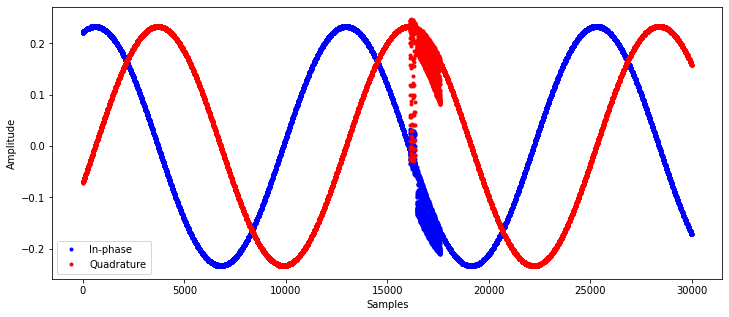
\includegraphics[scale=0.55]{figures/concepts_IQ-signal.png}
  \caption{In-phase and quadrature signals}
  \label{fig:iq-signal}
\end{figure}

To finish this introduction to SDR, we will describe the representation of the data. Figure \ref{fig:iq-signal} shows a graph of the samples returned by the SDR pipeline as dots. As can be seen, the signal is represented using two components. The "quadrature" component is shifted by 90 degrees in relation to the "in-phase" component. Every sample can be represented by a complex number where the real part adds to the in-phase component and the imaginary part adds to the quadrature component. Such a representation allows us to get a lot more information from the signal. \cite{kuisma_iq, ossmann_software}

Here, the X axis represents the sample number (starting at 0) rather than a time value. The link between the sample number and the time elapsed is the sampling rate ($F_s$), expressed in number of samples per second (S/s). For example, considering a sampling rate of 3MS/s, figure \ref{fig:iq-signal} shows a signal over 10ms: $\dfrac{30000[S]}{3000000[S/s]} = 0.01[s]$.

In this document, we will often use the magnitudes representation of a signal. Said representation is built by taking the magnitude (or module) of each complex sample and plotting it. Figure \ref{fig:mag} shows the magnitudes of the samples in figure \ref{fig:iq-signal}.

\begin{figure}[htp!]
  \centering
  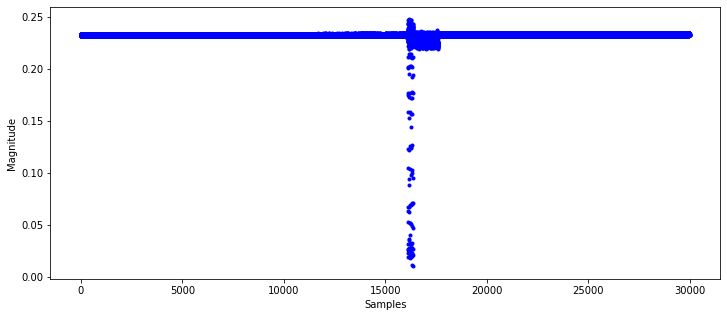
\includegraphics[scale=0.55]{figures/concepts_magnitudes.png}
  \caption{Signal represented as magnitudes}
  \label{fig:mag}
\end{figure}

% -------------------------------------------------------------------------------------------------------------
\subsection{Near-field communication} \label{nfc}

In order for our radio system to be effective, it needs to be adapted to the protocols used. This is why we need to understand how NFC operates.

NFC is the name for a group of communication protocols designed for small distance (max. 10cm) transactions. The idea is that a reader can supply power to a passive tag and get the information stored in it. The reader devices are sometimes called initiators or PCD (for Proximity Coupling Device) and the tags are sometimes called targets or PICC (for Proximity Inductive Coupling Card).

Operating at a frequency of 13.56MHz, NFC is well in the High Frequency (HF) range of 3 to 30MHz. This is substantially lower than most communication protocols like WiFi (2.4GHz or 5GHz), Bluetooth (2.4GHz) or ZigBee (868MHz, 915MHz or 2.4GHz).

Also in contrast to these other protocols, NFC's modulation scheme is On-Off Keying (OOK) which is a form of Amplitude Shift Keying (ASK). (Except for NFC type B, which uses BPSK in target to initiator mode.)

Because it is designed to work only in close proximity, NFC uses inductive coupling between devices to transmit information. In simple terms, this means the reader can only send a signal as far as its generated magnetic field goes. The passive tag responds by modulating the same magnetic field. It also means that interferences from radio devices operating in the same frequency range practically don't affect an NFC communication. \cite{wiki_near-field_2020}

\newpage

% State of the art
\section{State of the art} \label{sota}

\subsection{Taxonomy}

It is certainly useful to start with a review of the different ways to categorize the features and algorithms used by researchers in the field of radio frequency fingerprinting. More specifically, we'll focus on Radio Frequency Machine Learning (RFML) research, though other fingerprinting techniques exist that don't involve machine learning. The goal is to define our needs precisely and select the important factors to consider.

\subsubsection{Taxonomy for features} \label{features_tax}

The features we select must allow us to identify a precise device among potentially very similar devices. We need what \textcite{delgado_passive_2020} describe as a Physical Unclonable Function (PUF). PUFs are physical distortions that are unique to a specific system. They are another way of talking about fingerprints.

\textcite{xu_device_2015} propose three ways to categorize radio signal features:

\begin{itemize}
  \item based on the specificity of the feature (from vendor specific to device specific),
  \item based on the layers (PHY, MAC, Network and higher),
  \item and based on the acquisition method (passive or active).
\end{itemize}

Features from the MAC and higher layers typically require in depth knowledge of the protocols in play. Not only that, but they also tend to be less specific than we would like (either vendor specific or depending on the type of device). This indicates we should probably focus on the physical (PHY) layer features, which rely on imperfections in the manufacturing process of the devices.

\subsubsection{Taxonomy for fingerprinting algorithms} \label{algo-taxo}

\textcite{riyaz_deep_2018} provide a visual categorization of fingerprinting approaches, which we adapt in figure \ref{fig:algo-taxo}. We take a look at these approaches in the following paragraphs.

\begin{figure}[htp!]
  \centering
  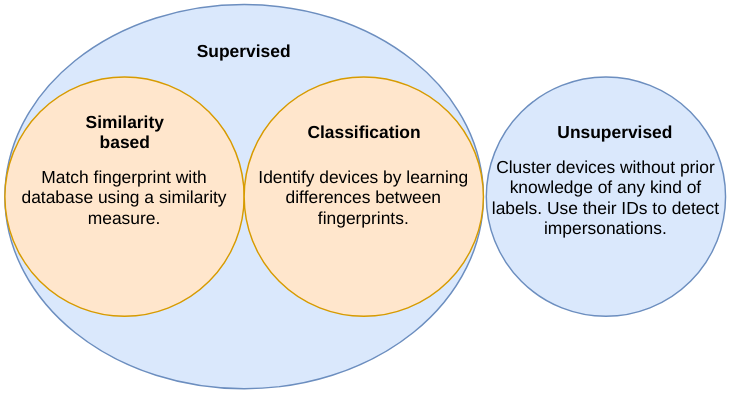
\includegraphics[scale=0.5]{figures/sota_algo-taxonomy.png}
  \caption{Fingerprinting algorithms taxonomy}
  \label{fig:algo-taxo}
\end{figure}

\paragraph{Supervised approaches:} Supervised approaches use features from labelled data to generate a function capable of separating the different classes. These approaches can be further categorized in similarity based and classification techniques.

Similarity based techniques are white-list algorithm that use a database of fingerprints and a similarity measure to determine whether a device is legitimate. Developing a technique like this usually requires prior knowledge of vendor specific device features \cite{riyaz_deep_2018}.

Classification systems can also require deep knowledge of the features and protocols used, in the case of "traditional", manually tuned classifiers. Those are built to extract predetermined features and work similarly to other white-list algorithms afterwards.

In this age of deep learning though, research seems to be more interested in classification techniques that are able to extract the features they need by themselves. This can be done through deep Multi-Layer Perceptrons (MLP) \cite{delgado_passive_2020, stankowicz_complex_2019} or through more advanced techniques like Convolutional Neural Networks (CNN) \cite{riyaz_deep_2018, oyedare_estimating_2019, youssef_machine_2017, morin_transmitter_2019, sankhe_no_2019}. The latter have proved very powerful in domains like computer vision, natural language processing and recommendation systems. This success is one of the reasons experimentations on CNNs are common in RFML research.

\paragraph{Unsupervised systems:} Unsupervised approaches cannot by themselves discriminate a legitimate device from an illegitimate one. They don't have that information, since they work with unlabeled data. In order to detect attempts of impersonation, such a system has to keep a record of fingerprints and linked identifiers (MAC addresses, serial numbers...). It can then throw an alert and update a black-list when multiple fingerprints are linked to the same ID or when multiple IDs are linked to the same fingerprint \cite{xu_device_2015, nguyen_device_2011}.

\textcite{xu_device_2015} specify that unsupervised approaches are appropriate when the fingerprints of legitimate devices are not available.

% -------------------------------------------------------------------------------------------------------------
\subsection{Acquisition}

The vast majority of the research considered for this project uses USRP systems to record transmissions as raw I/Q signals. The number of devices can be anywhere from 5 to 500 (but most often less than 20). They all use data acquired from WiFi (802.11) or Zigbee (802.15.4) devices. \cite{riyaz_deep_2018, oyedare_estimating_2019, youssef_machine_2017, morin_transmitter_2019, sankhe_no_2019, nguyen_device_2011}

Some, like \textcite{sankhe_no_2019}, also describe how they add artificially induced impairments to simulated signals with MatLab. This is something we could also do, but it is secondary. The focus is on the creation of a robust dataset of real world transmissions between an NFC reader and tags.

Although it isn't specified as such in any of the considered articles, we can deduce that in order for the dataset to be robust, it needs to answer some basic criteria. The following list assumes the dataset will be used to train a machine learning model to discriminate between passive tags.

\begin{itemize}
  \item It should contain recordings of both very similar and very different devices.
  \item The data transmitted should not be a discriminating factor.
  \item The number of devices should be high enough to analyse the scalability of the solution.
  \item Only one reader should be used to initiate a communication.
  \item Only one SDR should be used to capture the data.
  \item The capture's parameters should be constant across captures.
  \item At the same time, some variability in the signal's amplitude and phase may help the solution to be more general.
\end{itemize}

% -------------------------------------------------------------------------------------------------------------
\subsection{Features}

\subsubsection{Features selection}

Even if we don't plan to manually select and extract the features that will form the fingerprints of our devices, it is useful to learn about them. It will allow us to make sure they are present for the algorithm to extract and also allow us to design preprocessing methods that magnify the features.

Whether we end up with a system that is able to identify many devices uniquely, or one that only tries to separate a specific device from the others, we will need device specific accuracy. We don't want to make relay attacks impossible only if the attacker doesn't use a device from the same vendor as the victim's device. This is why in section \ref{features_tax}, we concluded that the features we are most interested in are from the physical layer.

Because of their nature, these features should be appropriate no matter the protocol used. The following list is composed of features described by \textcite{riyaz_deep_2018} and also used in other works.

\begin{itemize}
  \item{I/Q imbalance:} The amplitude and the phase are not exactly the same on the in-phase and the quadrature signals, because of the imperfections in the quadrature mixers.
  \item{Phase noise:} When the baseband signal is up-converted to the carrier frequency, it is sensible to phase noise which creates rotational vibrations.
  \item{Carrier frequency offset:} The difference between the carrier frequency of the transmitter and the carrier frequency of the receiver.
  \item{Harmonic distortions:} The Digital-to-Analog Converters (DAC) cause harmonic distortions because of imperfections.
\end{itemize}

\subsubsection{Preprocessing}

It is clear that preprocessing the data appropriately can greatly increase the accuracy of a model and reduce its complexity.

The first question to ask is how should the data be partitioned, in order to be fed to the learning algorithm. This question will be discussed in section \ref{nn-architecture} since it is identical to choosing the input of our model.

Several works mention wavelet transforms (either discrete or continuous) as effective means to amplify the characteristic features of a wireless device \cite{xu_device_2015, oyedare_estimating_2019, youssef_machine_2017}. They report increased accuracy and scalability, and reduced complexity. It is certainly worth it to explore this preprocessing method.

% -------------------------------------------------------------------------------------------------------------
\subsection{Machine learning applied to radio frequency}

\subsubsection{Challenges} \label{challenges}

\textcite{riyaz_deep_2018} highlight some of the challenges faced when working on RFML problems. They are reformulated in the three first items of the list below. The next items are personal additions.

\begin{enumerate}
  \item \label{itm:chall1} Finding the optimal partition length to feed the learning algorithm.
  \item \label{itm:chall2} Finding the optimal network architecture for the problem (in the case of neural networks).
  \item \label{itm:chall3} The absence of standard datasets to train and evaluate a model.
  \item Finding a cheap preprocessing method that improves performance and reduces complexity.
  \item Achieving a demonstrably scalable system.
\end{enumerate}

Great insight into item \ref{itm:chall1} is given by \textcite{youssef_machine_2017}. Indeed, they compare the performance of models trained with different input segment sizes. We delve deeper into this matter as well as item \ref{itm:chall2} in section \ref{nn-architecture}.

Item \ref{itm:chall3} is the core matter of the first part of our project. Indeed a considerable portion of our work consists in the elaboration of a dataset of NFC transmissions for different PICC devices.

\subsubsection{Supervised or unsupervised}

The aim of this project is to explore supervised learning techniques. This is why most of the literature considered here studies supervised systems. Also, in general, it seems works that use supervised methods are a lot more abundant than their unsupervised counterparts. This could be because of the popularity of models such as convolutional neural networks, and their apparent adaptability to the problem of RF fingerprinting.

Despite this, we can see that unsupervised learning techniques are also showing promising results. An example of this is the work of \textcite{nguyen_device_2011}. The paragraph about unsupervised systems in section \ref{algo-taxo} describes the basics of their system pretty well. They use a Nonparametric Bayesian model to detect the number of devices and then cluster them based on their fingerprints. This technique allows them to discriminate between an unknown number of devices that the model never encountered before. They show good results with four devices using two features strictly from the PHY layer.

While this work is interesting, it uses pre-engineered features. We were unable to find research on deep unsupervised learning techniques (such as deep belief networks) for the problem. Such a solution could be an interesting topic for another project.

\subsubsection{Comparing supervised approaches}

Several articles have compared the performance of different machine learning approaches. In the next paragraphs we discuss the findings of two of them.

\textcite{riyaz_deep_2018} compared their Convolutional Neural Network (CNN) with the techniques of Support Vector Machine (SVM) and logistic regression. They report substantially higher performance using their CNN (up to 60-70\% better accuracy). Their results, although limited in the number of devices (they only classify up to five), also seem to show that CNNs are more scalable than the other methods. Indeed, increasing the number of classes caused a significant drop in the performance of the other algorithms, but not for the CNN.

\textcite{youssef_machine_2017} compare the performance of four supervised algorithms: SVM, Deep Neural Networks, CNN and Accelerated Levenberg-Marquardt Multi-Stage Training (A-LM MST). The latter is an advanced classification technique that makes training deep neural networks less resource heavy by using a hierarchy of smaller Multi-Layer Perceptrons (MLP) rather than one big MLP. They use data collected from 12 WiFi transmitters.

Their results show impressive performance for their MST, especially when provided with very little data. Their CNN model is close second, although it performed significantly worse with very little data. Then comes the DNN with pretty good results and then only the SVM.

These results can guide us in our choices of experimentation. They show that SVM algorithms, while capable to some extent, are not appropriate for this specific problem. They also show CNNs are very promising, more scalable and more adaptable than "simple" DNNs. The MST solution is very interesting, but reducing the computational complexity is not our primary concern and the improvement doesn't seem that substantial.

\subsubsection{Neural network architectures} \label{nn-architecture}

In section \ref{challenges}, we noted that one of the challenges we face is to find the optimal partition length for the input of our model. To give an element of answer, \textcite{youssef_machine_2017} don't only compare the performance of 4 different models, they also do it with five different partition sizes (32, 64, 128, 256 and 512). They find their DNN architecture handles short segments better than long ones, while their CNN gets progressively more performant as the segments get larger.

\textcite{stankowicz_complex_2019} compare different kinds of formats for their inputs: two real valued series (one for the I component and one for the Q component), one complex valued series and one complex valued series with a spectrogram added as additional information. Their results are not the clearest, but they seem to show better performance when using a single series of complex values as input. They also show better performance in general for models that use complex valued weights. This is an interesting argument that we could explore.

Another of the challenges previously noted is finding the optimal architecture for a neural network in the context of RF fingerprinting. Studying the various architectures employed in previous works can help us define what is effective and what direction to take for our own experiences. We won't describe specific architectures in this section, but will reference elements from them when conceiving our experiments.

In general, the works cited throughout this section train their models to output the ID of a specific device. In this project, we would like to try training our model to simply discriminate between a legitimate device and the others. Elements like incremental learning (the ability to train the model again with more devices without starting from zero) and shift invariance (the ability not to care about the position of values in the input) are also important to take into consideration.

\newpage

% Dataset creation
\section{Dataset creation}

The first step of any classification project, especially if it uses machine learning, is to acquire and refine data. At the time the project was proposed, it was already clear that no existing dataset would be available. This proved to be true as discussed in section \ref{sota}, where we saw that existing research focuses on WiFi and Zigbee technologies.

% -------------------------------------------------------------------------------------------------------------
\subsection{Radio setup}

This section's goal is to describe the material used to capture the communications between NFC readers and tags. The final setup is illustrated in figure \ref{fig:radio-setup}.

\begin{figure}[htp!]
  \centering
  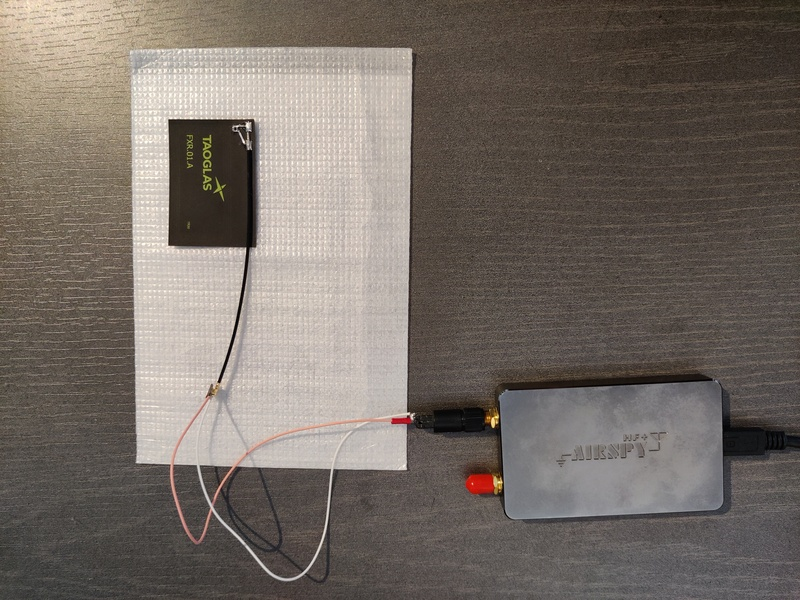
\includegraphics[scale=0.35]{figures/data_sdr-setup2.jpg}
  \caption{Airspy HF+ and antenna setup}
  \label{fig:radio-setup}
\end{figure}

\subsubsection{The SDR}

The first part of the analysis phase was conducted using a LimeSDR Mini\footnote{\url{https://www.crowdsupply.com/lime-micro/limesdr-mini}}. We used it to learn about SDR in general and to make our first recordings. In that regard it was very useful, but our model had a set of shortcomings we weren't able to accommodate. First, it became very hot very quickly, which couldn't have been good for the stability of the recording. Also, while it worked all the time for higher frequencies, it seemed to only pick up our HF signals one out of six times or so. This proved quite frustrating and attempts at tweaking the parameters in LimeSuite GUI (the device's official configuration software) generally resulted in errors.

Despite these setbacks, we were able to record communications well enough to decode the reader's transmissions, as described in section \ref{validation}. The tag's response, though, was drowned in the noise most of the time, as far as we can tell. These are the reasons why we replaced the LimeSDR Mini with the Airspy HF+\footnote{\url{https://airspy.com/airspy-hf-plus}} you can see in figure \ref{fig:radio-setup}, courtesy of Mr Joël Conus.

The Airspy HF+, as its name suggests, is built for HF (the frequency range in which NFC operates). As such, it proved a lot more stable at 13.56MHz (picking up our signal every time) and a lot less prone to heating. Most importantly, the noise level is much lower with this device, which allows us to clearly distinguish a tag's response. The only drawback is its sampling rate which can only be set at one of five values, the highest of which is 768kS/s. \cite{rtlsdr_our_2017, marks_airspy}

\begin{table}[h!]
  \centering
  \begin{tabular}{|l|l|l|l|}
    \hline
    \textbf{Name}         & \textbf{Frequency range}                                                       & \textbf{Bandwidth}                                           & \textbf{Transmitter?} \\ \hline
    \textbf{LimeSDR Mini} & 10MHz - 3.5GHz                                                                 & Up to 30.72 MHz                                                                  & Yes                        \\ \hline
    \textbf{Airspy HF+}   & \begin{tabular}[c]{@{}l@{}}HF: 9kHz - 31MHz\\ VHF: 60MHZ - 260MHZ\end{tabular} & \begin{tabular}[c]{@{}l@{}}768kHz, 384kHz, 192kHz,\\ 96kHz or 48kHz\end{tabular} & No                         \\ \hline
  \end{tabular}
  \caption{Theoretical characteristics of mentionned SDRs}
  \label{tab:pcd-inventory}
\end{table}

\subsubsection{The antenna}

As described in section \ref{nfc}, NFC uses inductive coupling rather than the more common far-field electromagnetic radiations. Because of this, our system needs a near-field antenna, which in this case is really just an inductor. A simple loop of copper wire qualifies as such, but in order for our system to be perfectly tuned to 13.56MHz, we used an industrial antenna: the Taoglas FXR.01.A\footnote{\url{https://www.taoglas.com/product/fxr01-nfc-flex-reader-antenna}}.

The antenna should be placed at least 15mm away from metallic objects, for they interfere with the magnetic field used for the communication.

As can be seen in figure \ref{fig:radio-setup}, the adapter between the SDR and the antenna is homemade using spare connectors and copper wires. The risk of interferences because of this rather unsophisticated adapter is noted, but doesn't seem to be significant later in the work.

% -------------------------------------------------------------------------------------------------------------
\newpage
\subsection{Inventory of devices}

Here, we list the devices used to create the dataset. These include the PCDs (readers) and the PICCs (tags) whose communications were captured.

In terms of readers, table \ref{tab:pcd-inventory} lists the few devices used, for documentation purposes. Of course, only one reader will be used to elaborate the final dataset, but it was useful to compare the results during the analysis phase. We weren't able to find a specific NFC chip in either smartphone's characteristics. The final dataset will be created with the help of \texttt{reader1}, as it is more recent.

\begin{table}[h!]
  \centering
  \begin{tabular}{|l|l|l|}
    \hline
    \textbf{Name}    & \textbf{Type} & \textbf{Model} \\ \hline
    \textbf{reader1} & Smartphone    & OnePlus 8      \\ \hline
    \textbf{reader2} & Smartphone    & Nokia 7+       \\ \hline
  \end{tabular}
  \caption{Inventory of PCD devices}
  \label{tab:pcd-inventory}
\end{table}

On the other hand, the list of tags and their technical details can be found in table \ref{tab:picc-inventory}. A picture of tags 1 to 7 is also provided in figure \ref{fig:tags}. As the table shows, tags 1 to 5 use the exact same chip model. Tags 1 to 8 are all NFC type A compliant, while tag 9 uses the FeliCa standard from Sony. It will be interesting to contrast the classification performance between tags of the same type and between tags of different types.

\begin{table}[h!]
  \centering
  \begin{tabular}{|l|l|l|l|l|l|l|}
    \hline
    \textbf{Name} & \textbf{NFC type} & \textbf{Standard} & \textbf{Chip}     & \textbf{Writable} & \textbf{Storage} & \textbf{Bit rate} \\ \hline
    \textbf{tag1} & NFC-A             & ISO 14443-3A      & NTAG213           & Yes               & 137B             & 106kb/s         \\ \hline
    \textbf{tag2} & NFC-A             & ISO 14443-3A      & NTAG213           & Yes               & 137B             & 106kb/s         \\ \hline
    \textbf{tag3} & NFC-A             & ISO 14443-3A      & NTAG213           & Yes               & 137B             & 106kb/s         \\ \hline
    \textbf{tag4} & NFC-A             & ISO 14443-3A      & NTAG213           & Yes               & 137B             & 106kb/s         \\ \hline
    \textbf{tag5} & NFC-A             & ISO 14443-3A      & NTAG213           & Yes               & 137B             & 106kb/s         \\ \hline \hline
    \textbf{tag6} & NFC-A             & ISO 14443-3A      & Mifare Classic 1k & Yes               & 716B             & 106kb/s         \\ \hline
    \textbf{tag7} & NFC-A             & ISO 14443-3A      & Mifare Classic 1k & Yes               & 716B             & 106kb/s         \\ \hline \hline
    \textbf{tag8} & NFC-A             & ISO 14443-4       & Mifare Classic 4k & No                & \~4kB            & 106kb/s         \\ \hline
    \textbf{tag9} & FeliCa            & JIS 6319-4        & RC-S967           & No                & 208B             & 212kb/s         \\
                  &                   &                   &                   &                   &                  & 424kb/s         \\ \hline
  \end{tabular}
  \caption{Inventory of PICC devices}
  \label{tab:picc-inventory}
\end{table}

On the PICCs that are marked writable, the content is harmonized to ensure the algorithm won't use the content as a feature to identify devices.

\begin{figure}[htp!]
  \centering
  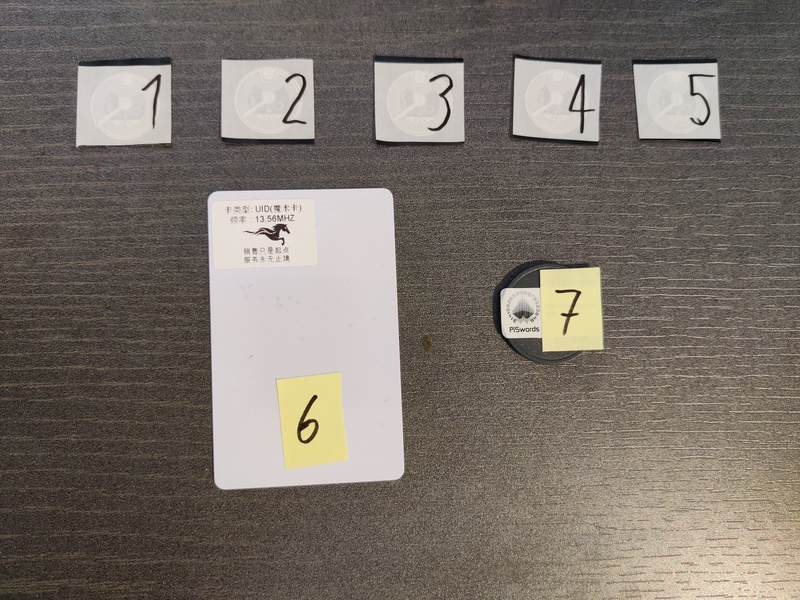
\includegraphics[scale=0.35]{figures/data_standard-tags2.jpg}
  \caption{NFC tags 1-7}
  \label{fig:tags}
\end{figure}

\subsubsection{Software used}

\textbf{EXPAND A LITTLE, TALK ABOUT SYSTEM?}

We used GNU Radio Companion (GRC)\footnote{\url{https://wiki.gnuradio.org/index.php/Main_Page}} for all of our experiments. It is a very versatile tool, allowing us to define software pipelines using a block interface to create flow graphs. As it compiles to python, the idea is to use it as a base for acquisition and processing scripts.

The format used by GRC's file writer is simple. It writes raw bytes into a file, alternating between the real part and the imaginary part of the sample. Both parts are written as 32 bits floating-point numbers.

On the reader (an Android smartphone), we use the NFC Tools\footnote{\url{https://www.wakdev.com/en/apps/nfc-tools.html}} app to get information about the tags and manipulate their content.

% -------------------------------------------------------------------------------------------------------------
\subsection{Dataset description}

\subsubsection{Requirements}

In order for the dataset to be robust, it needs to answer some basic criteria. The following list assumes the dataset will be used to train a machine learning model to discriminate between passive tags.

\begin{itemize}
  \item It should contain recordings of both very similar and very different devices.
  \item The data transmitted should not be a discriminating factor.
  \item The number of devices should be high enough to analyse scalability and generalization.
  \item Only one reader should be used to initiate a communication.
  \item Only one SDR should be used to capture the data.
  \item The capture's parameters should be constant across captures.
\end{itemize}

If some of those items are not met, the model trained using this data could use the content of the tags or the capture's parameters to categorize the data. It may also be unable to generalize when unknown tags appear.

\textbf{VARIABILITY IS ALSO IMPORTANT}

\subsubsection{First dataset}

\textbf{DESCRIPTION FROM README}

This dataset was built while trying to introduce as little variability as possible. The positions of the tags and reader was kept as similar as possible between recordings. Each recording was made using `scripts/acquisition/capture.py` with `--time 3`.

\begin{itemize}
  \item 3 recordings of each of the 9 tags
  \item Length of a recording: 3 seconds
  \item Number of samples per recording: 3 * 768'000 = 2'304'000 samples
  \item (Content of tags 1 through 7: 36B of the 'A' character.)
\end{itemize}

\subsubsection{Visualization of the signal}

A typical NFC communication, captured using the hardware described above, is represented in figure \ref{fig:nfc-full}. We can observe that before the reader is brought to the tag, the line is almost flat at zero. This shows a very low noise level. Then, there is a sudden surge of amplitude in the signal as the reader generates the magnetic field required for the communication. This part, referred to as the "transient portion" of the signal by \textcite{xu_device_2015} (although they talk about WiFi), might be very characteristic of the device. Then, the amplitude decreases and regular request/responses start.

\begin{figure}[htp!]
  \centering
  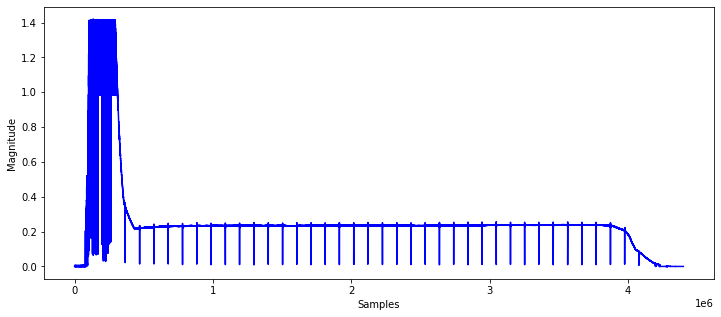
\includegraphics[scale=0.5]{figures/data_whole-transmission.png}
  \caption{NFC communication represented as magnitudes}
  \label{fig:nfc-full}
\end{figure}

In figure \ref{fig:nfc-single}, we take a closer look at one of the request/responses of the previous figure. We can clearly see a first transmission followed by a pause and then a second transmission, with smaller amplitude. This is how NFC communications work, with a request sent by the reader device followed by the tag's response through modulation of the reader's magnetic field.

\begin{figure}[htp!]
  \centering
  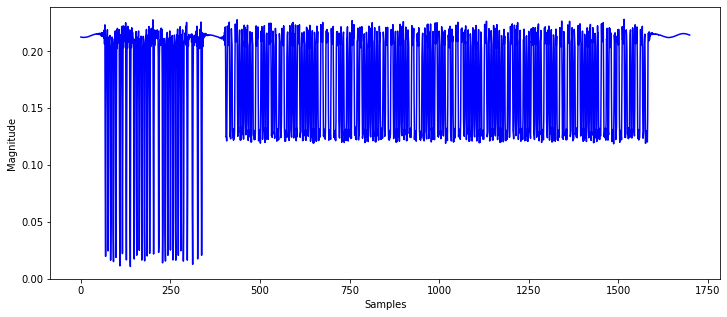
\includegraphics[scale=0.5]{figures/data_single-request-response.png}
  \caption{NFC single request/response represented as magnitudes}
  \label{fig:nfc-single}
\end{figure}

% -------------------------------------------------------------------------------------------------------------
\subsection{Validating the dataset} \label{validation}

\textbf{FIRST, VISUALIZE. THEN, DECODE to make sure we have the data from the tag and the reader. THEN MEASURE TOOLS}

The next step in the elaboration of the dataset is to be absolutely sure that the data is fully captured by our setup. The previous section seems to show this is the case, but to be sure we would need to decode the signal.

To do so, we need to know the modulation and coding used by the protocol. In the case of our NFC-A tags, the reader's transmissions are coded with a modified Miller code, while the tag's responses are coded with Manchester coding. Both modulate the data with On-Off Keying (OOK), which represents zeroes as no change of amplitude and ones as changes in amplitude over a given time period. \cite{wiki_off_2020}

Miller coding, as applied in NFC communications, works by mapping four symbols in the signal to a bit. A one is always coded as "high, high, low, high" or 1101. A zero can be coded as 0111 or 1111, depending on whether it came after a zero or a one respectively. \cite{phy_nfc_coding}

Manchester coding on the other hand, uses transitions to express bits. High-to-low stands for a one and low-to-high represents a zero. This only takes into account transitions that happen at the middle of a period. Transitions at the start of a period don't matter. \cite{phy_nfc_coding, wiki_manchester_2019}

Using \textcite{rona_sniffing_2017}'s GNU Radio Companion module \texttt{gr-nfc}\footnote{\url{https://github.com/jcrona/gr-nfc}}, we were able to decode messages coming from the reader. An excerpt of the decoded requests issued to tag1 is shown in figure \ref{fig:decoded}. They show typical NFC requests like 52 (wake up), 50 00 (HALT) or 93 and 95 which are anticollision requests. The figure also shows tag1's UID is present in the anticollision requests, using a screenshot of the tag's properties.

\begin{figure}[htp!]
  \centering
  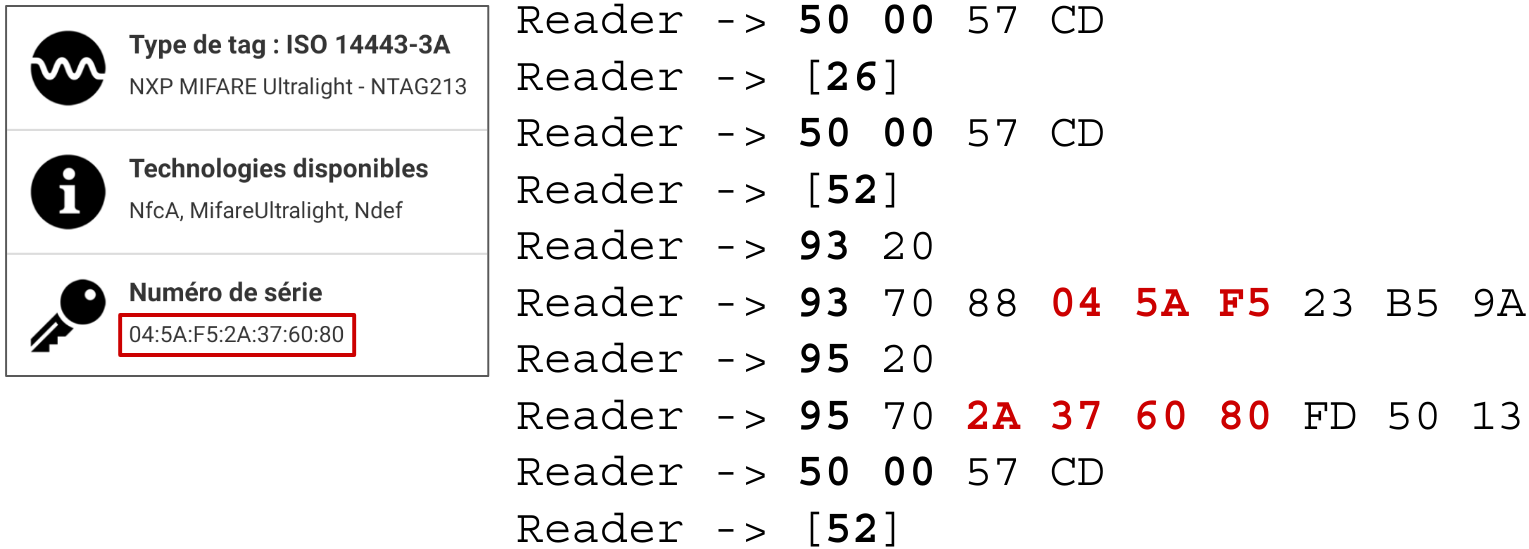
\includegraphics[scale=0.35]{figures/data_decoded-frames_app.png}
  \caption{Decoded frames from the reader, showing tag1's UID in red}
  \label{fig:decoded}
\end{figure}

At the time of this writing, we are investigating ways to decode the transmissions of both the reader and the tags. Using \texttt{sigrok}'s decoders\footnote{\url{https://sigrok.org/wiki/Protocol_decoders}} or Universal Radio Hacker\footnote{\url{https://github.com/jopohl/urh}}, we should be able to at least validate the signals, and maybe even decode them fully.

% -------------------------------------------------------------------------------------------------------------
\subsection{More complete dataset}

\textbf{TBC}

\newpage

% Data preparation
\section{Data preparation}

Once the dataset is captured and stored, the data still has to be formatted and prepared to be fed to our models. We decided to alter the recordings as little as possible, since it is very valuable to have raw data in projects like this one. This means any modification of the data is done at runtime. This section describes the formatting and preprocessing applied to the datasets.

\subsection{Environment}

We used python to work with our datasets and to write the models described in next section. Visualizations were done in \texttt{Jupyter notebooks} using \texttt{matplotlib}. Data processing was achieved in a python project using \texttt{numpy} to read and manipulate the data and \texttt{scipy}'s signal processing library.

% -------------------------------------------------------------------------------------------------------------
\subsection{Data partitioning}

\subsubsection{Raw partitioning}

Our first approach with the datasets was to segment each recording in windows of size $n$. Inspired by \textcite{youssef_machine_2017}, we made the window size a parameter, so that we could tune it.

The result for each tag is an array of windows, each comprised of $n$ complex samples. If the number of samples in a tag's recordings is of size $L$, then this array contains $L/n$ windows.

\subsubsection{Detecting communications}

It was soon clear that feeding the raw data without at least selecting segments that actually contained communications would not yield fantastic results. Indeed, most windows would contain only the carrier signal generated by the reader. These long segments of the signal contain little to no meaningful information. This is why we used peak detection algorithms to detect actual communications and filter out the uninteresting parts of the signal.

\begin{figure}[htbp!]
  \centering
  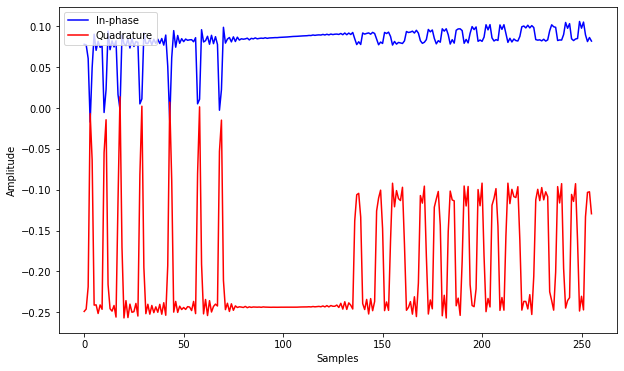
\includegraphics[scale=0.55]{figures/dataprep_window.png}
  \caption{Visual example of a window of size $n = 256$}
  \label{fig:window}
\end{figure}

\textbf{Do we use height or prominence?} An example of a resulting window can be seen in figure \ref{fig:window}.

\subsection{Input formatting}

Once our data is filtered and partitioned for input, the question of the format comes up. Indeed, a machine learning model will not accept complex numbers as input without adapting the loss function. This can be done without great difficulty, but most of the research we considered preferred representing the data as a two-dimensional array comprised of two float arrays: one for the real parts and the other for the imaginary parts. Figure \ref{fig:2din} shows a representation of the input after the windows were created and formatted this way.

\begin{figure}[htbp!]
  \centering
  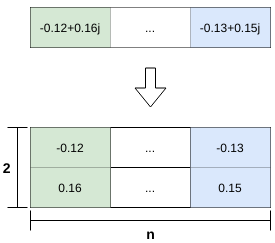
\includegraphics[scale=0.75]{figures/dataprep_2d.png}
  \caption{Format for the two-dimensional input}
  \label{fig:2din}
\end{figure}

For our experiments with SVMs, such a representation wasn't appropriate since SVMs don't accept multidimensional inputs. This is why we propose two formatting options: "2D" for the neural networks and "1D" for the SVM. The latter appends the array containing the imaginary parts to the array containing the real parts, as shown in figure \ref{fig:1din}.

\begin{figure}[htbp!]
  \centering
  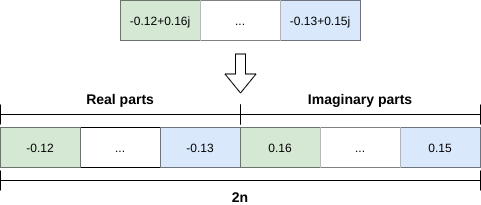
\includegraphics[scale=0.75]{figures/dataprep_1d.png}
  \caption{Format for the simple input}
  \label{fig:1din}
\end{figure}

% -------------------------------------------------------------------------------------------------------------
\subsection{Preprocessing}

normalization (amplitude, detrending?)

CWT

\newpage

% Machine learning models and experiences
\section{Machine learning}

\subsection{Environment}

python libraries, hardware, etc.

\subsection{Data formatting}

segments, etc

\subsection{Model architecture}

Youssef as first

Riyaz then maybe

Complex?

\subsection{Experiments with dataset 1}

Small dataset, simple, airspy HF+

\subsubsection{SVM}

\subsubsection{CNN}

Might not have enough information in signal...


\textbf{Test model with WiFi dataset??????}

\newpage

\section{Conclusion}

During this project, we have achieved tasks as varied as the elaboration of an acquisition setup for radio waves, attempts at decoding a modulated signal, signal processing, data manipulation, and building deep learning models.

Despite our best efforts to try as many things as possible, we have only scratched the surface of the theme of radio frequency machine learning. There are many elements we would have loved to explore: data preprocessing methods like wavelet transforms, dataset augmentation through sliding windows, complex weighted neural networks, unsupervised techniques, etc. These topics will have to be left to future work, as this project comes to an end.

Our results, while not overwhelming, are reasonably good and gave us reasons to believe the task to be feasible. We are able to give elements of answers and open paths for future development.

\newpage

% Bibliography
\printbibliography[heading=bibintoc, title={Bibliography}]
\newpage

% Annexes

% Work journal

\end{document}
